O parâmetro $L_e$ é o comprimento equivalente, que depende da composição da estrutura, como abaixo:

\begin{figure}[H]
	\begin{center}
	\caption{Comprimento equivalente de um pilar.}
    	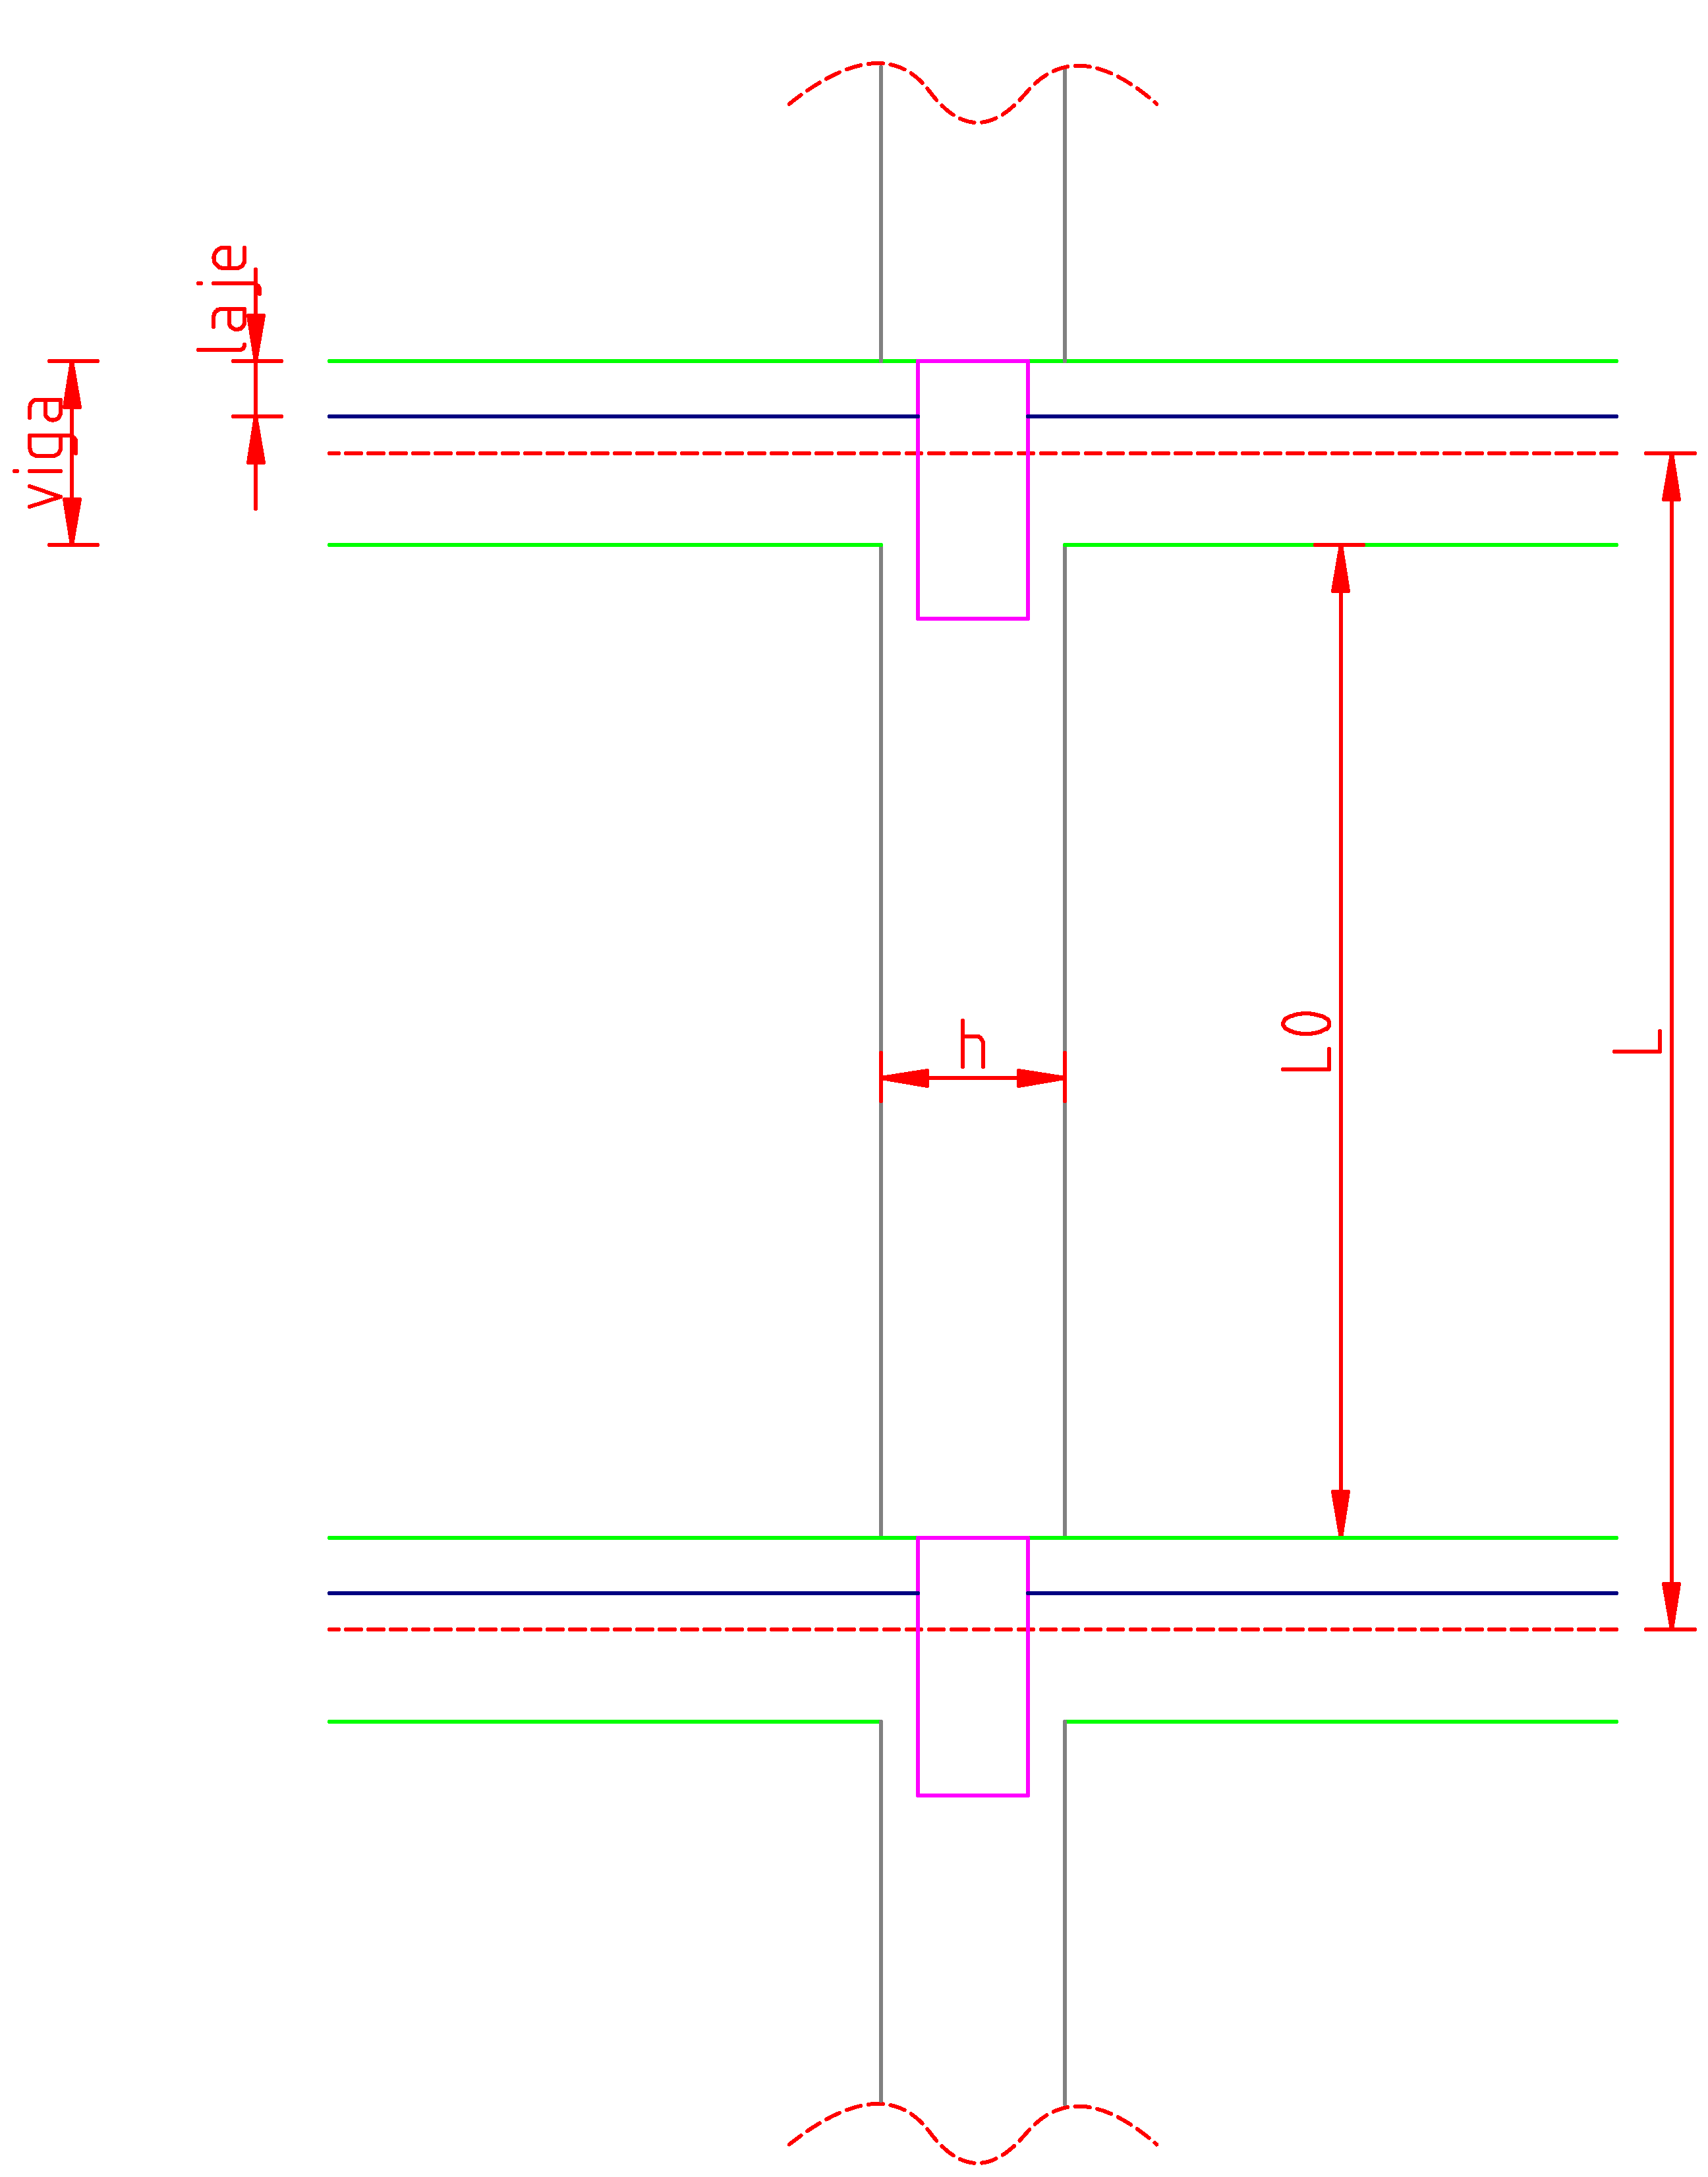
\includegraphics[width=0.7\textwidth]{Comprimento-equivalente/Imagens/Comprimento-equivalente.png}
	\end{center}
\end{figure}

\begin{equation}
	\label{equacao-comprimento-equivalente}
	L_e\leqslant\left\{
		\begin{array}{ll}
		L_0+h \\
		L
		\end{array}\right.
\end{equation}

Onde $L_0$ é a distância entre faces internas dos elementos estruturais, supostos horizontais, que vinculam o pilar, ou seja, a distância do topo da viga inferior à base da viga superior; $h$ é a dimensão da seção transversal do pilar, medida no plano da estrutura em estudo (eixo $x$ e $y$); e $L$ é a distância entre os eixos dos elementos estruturais aos quais o pilar está vinculado (distância do eixo da viga inferior ao eixo da viga superior).

\textbf{Exercício}: Definir o comprimento equivalente do pilar abaixo para as direções $x$ e $y$, considerando a seguinte figura para um pilar P1(35x60):

\begin{figure}[H]
	\begin{center}
	\caption{Configuração de um pilar genérico P1 .}
    	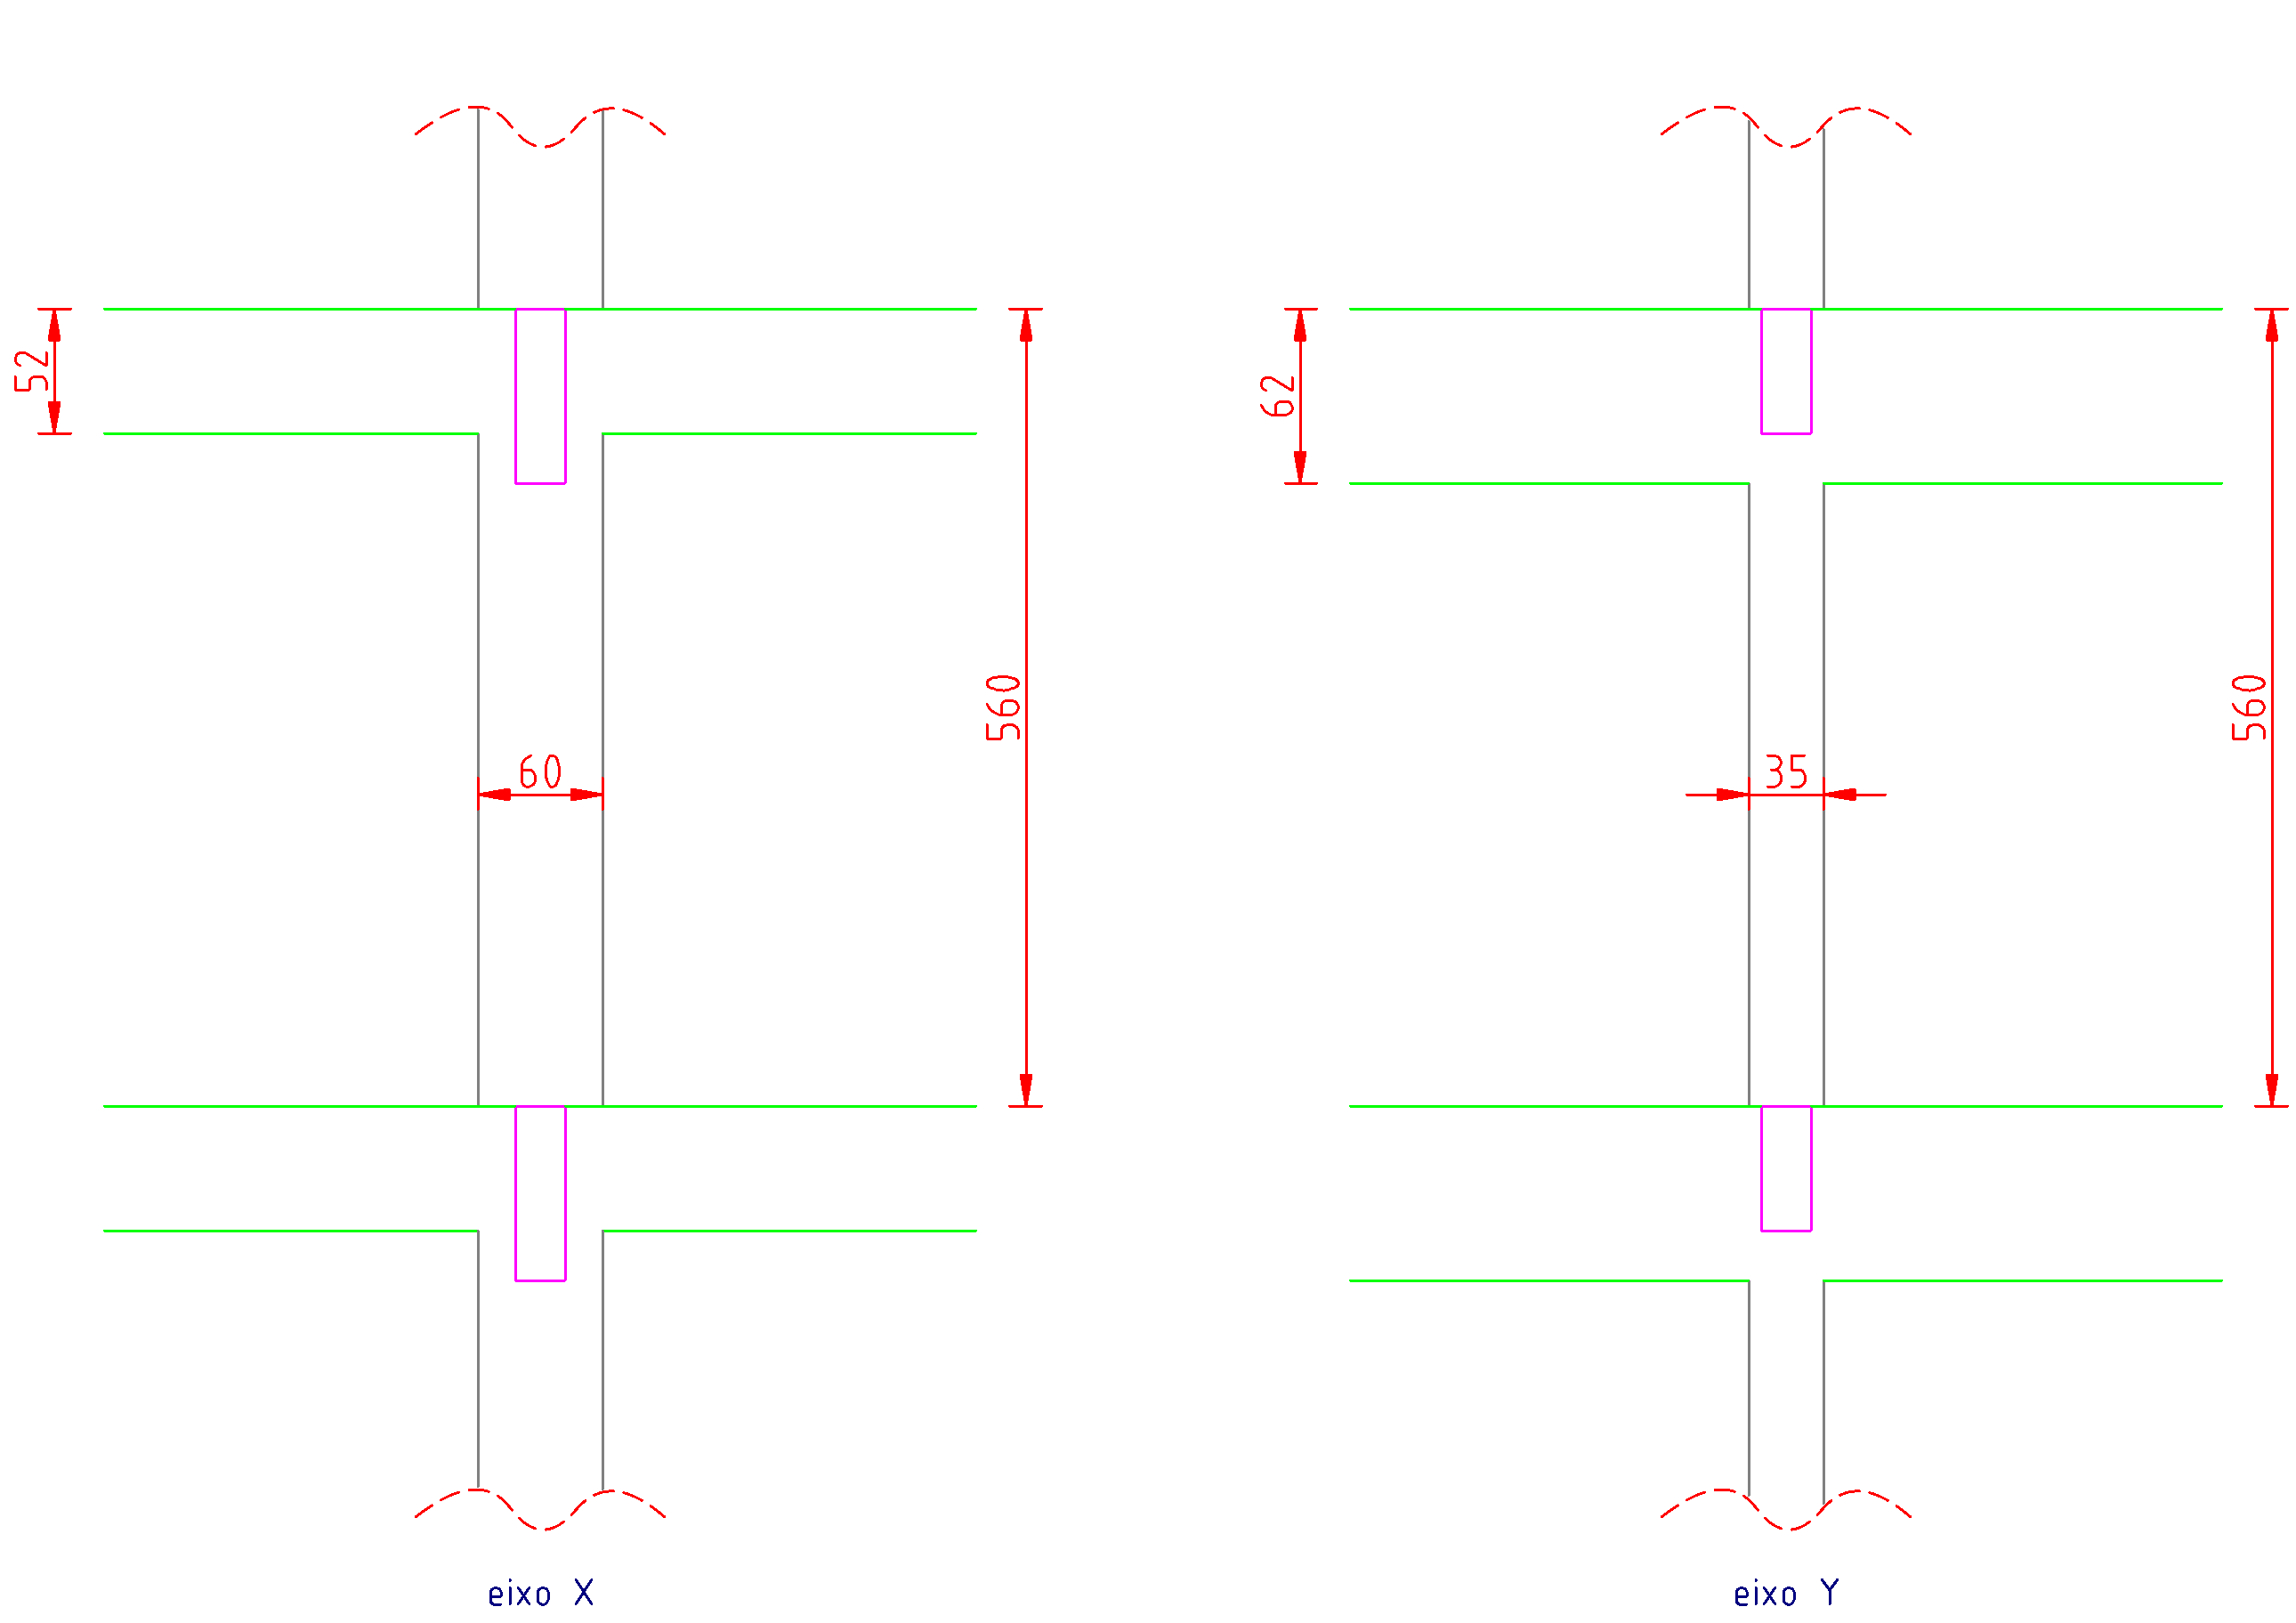
\includegraphics[width=0.85\textwidth]{Comprimento-equivalente/Imagens/Comprimento-equivalente-exercicio.png}
	\end{center}
\end{figure}
$$
	L_{e,\;x}\leqslant\left\{
		\begin{array}{ll}
		L_0+h=(560-52)+60=568\;cm \\
		L=\textbf{560\;cm}
		\end{array}\right.
$$
$$
	L_{e,\;y}\leqslant\left\{
		\begin{array}{ll}
		L_0+h=(560-62)+35=\textbf{533\;cm} \\
		L=560\;cm
		\end{array}\right.
$$

